\documentclass[11pt]{article}

\usepackage{graphicx}
%\usepackage{algorithmic}
%\usepackage{algorithm}
\usepackage{amssymb}
\usepackage{amsmath}
\usepackage{enumerate}
\usepackage[mathscr]{euscript}

\begin{document}

\pagenumbering{arabic}

\begin{center}
{\LARGE{\textbf{Computational Theories of Collaboration}}} \\
\Large\textsc{Ph.D. Comprehensive Exam} \\[1em]
\large\textnormal{Mohammad Shayganfar - mshayganfar@wpi.edu} \\
\large\textnormal{May, 26 2015}
\end{center}

\section{Introduction to Collaboration Theories}

The construction of computer systems and robots that are intelligent,
collaborative problem-solving partners is important in Artificial Intelligence
(AI) and its applications. It has been always important for us to make computer
systems better at helping us to do whatever they designed for. To build
collaborative systems, we need to identify the capabilities that must be added
to individual agents so that they can work with us or other agents. As Grosz
says, collaboration must be designed into systems from the start; it cannot be
patched on \cite{grosz:collaborative-systems}.

Collaboration is a special type of coordinated activity in which the
participants work jointly, together performing a task or carrying out the
activities needed to satisfy a shared goal \cite{grosz:collaboration}.
Collaboration involves several key properties both in structural and functional
levels. For instance, most collaborative situations involve participants who
have different beliefs and capabilities; most of the time collaborators only
have partial knowledge of accomplishing the collaborative activities;
collaborative plans are more than the sum of individual plans; collaborators
require to maintain mutual beliefs about their shared goal through out the
collaboration; they need to be able to communicate with others effectively;
they need to commit to the group activities and to their role in it;
collaborators need to commit to the success of others; they need to reconcile
between commitments to existing collabortion and their other activities;
and they need to interpret others' actions and utterances in the collaboration
context \cite{grosz:mice-menus}. These collaboration properties are captured by
the existing computational collaboration theoriess.

As we mentioned, to be collaborative, partners, e.g., a robot and a human, need
to meet the specifications stipulated by collaboration theories. These theories
argue for an essential distinction between a collaboration and a simple
interaction or even a coordination in terms of commitments
\cite{grosz:shared-plans, lochbaum:collaborative-planning}. This document
briefly provides description of major computational collaboration theories,
their similarities and differences, and their application in AI and robotics. It
primarily focuses on Joint Intention, SharedPlans and hybrid theories of
collaboration. In this document, we do not present the theroies in formal
language, but simply describe their features in general terms.

\section{Computational Theories of Collaboration}

The prominent collaboration theories are mostly based on plans and joint
intentions \cite{cohen:teamwork} \cite{grosz:plans-discourse}
\cite{Litman:discourse-commonsense}, and they were derived from the BDI
paradigm developed by Bratman \cite{bratman:intentions-plans} which is
fundamentally reliant on folk psychology \cite{ravenscroft:folk}. The two
theories, Joint Intentions \cite{cohen:teamwork} and SharedPlans
\cite{grosz:plans-discourse}, have been extensively used to examine and describe
teamwork and collaboration.

The SharedPlans theory is based on the theories of Bratman and Pollack
\cite{bratman:plans-reasoning,pollack:plan-inference,
pollack:plan-mental-attitudes}, who outline a mental-state view of plans in
which having a plan is not just knowing how to do an action, but also having the
intention to do the actions entailed. Bratman's views of intention goes back to
philosophical views of Anscombe \cite{anscombe:intention} and
$Casta\tilde{n}eda$ \cite{castaneda:thinking} about intention. Also, as Grosz
and Sidner mention in \cite{grosz:plans-discourse} the natural segmentation of
discourse reflects intentional behaviors in each segment. These intentions are
designated as Discourse Segment Purposes (DSPs) which are the basic reasons for
engaging in different segments of discourse. DSPs are a natural extention of
Gricean intentions at the utterance level \cite{neale:grice-language}.

Cohen and Levesque also mention that in Joint Intentions theory their view of
intention is primarily future-directed \cite{cohen:intention-commitment} which
makes their view along with the Bratman's theory of intention
\cite{bratman:intention}, contra Searle \cite{searle:collective}.\\

\textbf{Commitment} -- One of the most important concepts of teamwork and
collaboration is the concept of commitment. Collaboration theories require to
meet the notion of commitment, otherwise the participants are just doing some
coordinated works. Since the prominent computational collaboration theories,
reviewed in this paper, are based on Bratman's view of intention, here we
briefly provide his view of commitment before describing these theories. Bratman
defines certain prerequisites for an activity to be considered shared and
cooperative \cite{bratman:shared-activity}. He stresses the importance of:

\begin{enumerate}[a)]
  \item \textbf{Mutual commitment to joint activity} -- which can be achieved by
  agreement on the joint activity, and preventing to abondon activity without
  involving teammates;
  \item \textbf{Mutual suppport} -- which can be achieved by team members
  if they actively try to help teammate activity;
  \item \textbf{Mutual responsiveness} -- which means team members should take
  over tasks from teammates if necessary.
\end{enumerate}

In the following sections, we are also going to see how each collaboration
theory addresses the notion of commitment.

\subsection{SharedPlans Theory}
\label{sec:sharedplans}

The SharedPlans model of collaborative action, presented by Grosz and Sidner
\cite{grosz:planning-acting, grosz:collaboration, grosz:plans-discourse}, aims
to provide the theoretical foundations needed for building collaborative
robots/agents \cite{grosz:collaborative-systems}. SharedPlans is a general
theory of collaborative planning that requires no notion of joint intentions
(see Section \ref{sec:joint-intentions}), accommodates multi-level action
decomposition hierarchies and allows the process of expanding and elaborating
partial plans into full plans (see Section \ref{sec:full-partial-plan}).
SharedPlans theory explains how a group of agents can incrementally form and
execute a shared plan that then guides and coordinates their activity towards
the accomplishment of a shared goal. SharedPlans is rooted in the observation
that collaborative plans are not simply a collection of individual plans, but
rather a tight interleaving of mutual beliefs and intentions of different team
members. In \cite{grosz:collaboration} Grosz and Kraus use first-order logic to
present the formalization of SharedPlans.

Grosz and Sidner in \cite{grosz:plans-discourse} present a model of plans to
account for how agents with partial knowledge collaborate in the construction of
a domain plan. They are interested in the type of plans that underlie discourse
in which the agents are collaborating in order to achieve a shared goal. They
propose that agents are building a shared plan (see Section \ref{sec:shared}) in
which participants have a collection of beliefs and intentions about the actions
in the plan. Agents have a library of how do their actions, i.e. recipes (see
Section \ref{sec:recipe}). These recipes might be partially specified as to how
an action is executed, or contributes to a goal (see Section
\ref{sec:full-partial-plan}). Then, each agent communicates their beliefs and
intentions by making utterances about what actions they can contribute to the
shared plan. This communication leads to the construction of a shared plan, as
well as terminating the collaboration with each agent mutually believing that
there exists one agent who is going to execute an action in the plan, and the
fact that that agent has intention to perform the action, and that each action
in the plan contributes to the goal \cite{grosz:plans-discourse}
\cite{lochbaum:plan-models}.

Later in Section \ref{sec:shared}, we are going to see that to successfully
complete a plan the collaborators must mutually believe that they have a common
goal and have agreed on a sequence of actions for achieving that goal. They
should believe that they are both capable of performing their own actions and
intend to perform those actions while they are committed to the success of their
plans.

\subsubsection{Recipes}
\label{sec:recipe}

The SharedPlans theory differentiates between knowing how to accomplish a goal
(a recipe) and having a plan, which includes intentions. The SharedPlans
definition of mutual beliefs states that when agents have a shared plan for
doing some action, they must hold mutual beliefs about the way in which they
should perform that action \cite{grosz:collaboration,grosz:plans-discourse}.
Following Pollack \cite{pollack:plan-mental-attitudes}, the term recipe refers
to what collaborators know when they know a way of doing an action. Recipes are
specified at a particular level of detail. Although, the agents need to have
mutual beliefs about actions specified in the recipe, they do not need to have
mutual beliefs about all levels of performing actions. Therefore, having mutual
belief of the recipe means that the collaborators hold the same beliefs about
the way in which an action should be accomplished. Consequently, the
collaborators need to agree on how to execute an action. Recipes are
aggregations of action-types and relations among them. Action-types, rather than
actions, are the main elements in recipes. Grosz and Sidner in their earlier
work \cite{grosz:plans-discourse} have considered only simple recipes in which
each recipe consisted of only a single action-type relation
\cite{lochbaum:plan-models}. Recipes can be partial, meaning thay can expand and
be modified over time.

\subsubsection{Shared Plans}
\label{sec:shared}

Grosz and Sidner propose that collaboration must have the following three
elements which also shows the importance of the shared plans:

\begin{enumerate}
  \item the participants must have commitment to the shared activity;
  \item there must be a process for reaching an agreement on a recipe for the
  group action;
  \item there must be commitment to the constituent actions. 
\end{enumerate}

\textit{Shared plan} is an essential concept in the collaboration context.
The definition of the shared plan is derived from the definition of plans
Pollack introduced in \cite{pollack:plan-inference,
pollack:plan-mental-attitudes} since it rests on a detailed treatment of the
relations among actions and it distinguishes the intentions and beliefs of an
agent about those actions. However, since Pollack's plan model is just a simple
plan of a single agent, Grosz and Sidner extended that to plans of two or more
collaborative agents. The concept of the shared plan provides a framework in
which to further evaluate and explore the roles that particular beliefs and
intentions play in collaborative activity \cite{lochbaum:plan-models}. However,
this formulation of shared plans (a) could only deal with activities that
directly decomposed into single-agent actions, (b) did not address the
requirement for the commitment of the agents to their joint activities, and (c)
did not adequately deal with agents having partial recipes
\cite{grosz:collaboration}. Grosz and Kraus in \cite{grosz:collaboration},
reformulate Pollack's definition of the individual plans
\cite{pollack:plan-mental-attitudes}, and also revise and expand the SharedPlans
to address these shortcomings.

Figure \ref{fig:plans} shows what we need to add to individual plans in order to
have plans for group actions. The top of the figure lists the main components
for individual plans. First, an individual agent needs to know the recipe for an
action, whereas agents in a group need to have a mutual belief of a recipe for
an action. In the case of a group plan, having mutual belief of a recipe, leads
the agents to agree on how they are going to execute the action. Then, just as
individual agents need to have the ability to perform the constituent actions in
an individual plan and must have intentions to perform them, the participants in
a group activity need to have individual or group plans for each of the
constituent actions in the mutually agreed recipe
\cite{grosz:collaborative-systems, grosz:plans-discourse}.

\begin{figure}[tbh]
  \center
  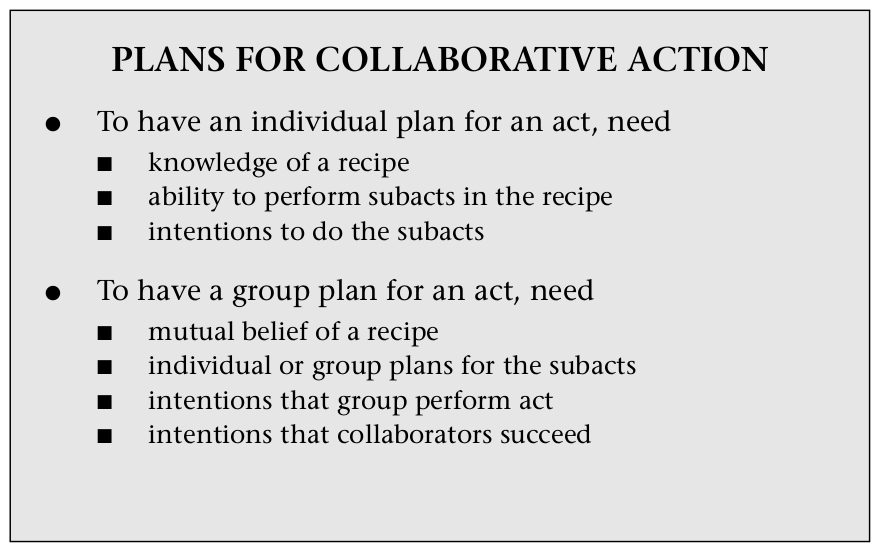
\includegraphics[width=0.9\textwidth]{figure/plans.png}
  \caption{Plans for collaborative action \cite{grosz:collaborative-systems}.}
  \label{fig:plans}
\end{figure}

As shown in Figure \ref{fig:plans} (bottom), plans for group actions include two
essential constituents that do not have correlates in the individual plan.
First, the agents need to have a commitment to the group activity; All the
agents need to intend that (see Section \ref{sec:intend-to-that}) the group will
do the action. For instance, a robot and an astronaut need to have intentions
that they install solar panels together. Among other things, these intentions
will keep them both working on the panels until the panels are installed.
Second, the participants need to have some commitment to the other agents to
succeed in their own their actions. For instance, the robot must have an
intention that the astronaut be able to measure the quality of installation
successfully. This intention will prevent the robot from interrupting the
astronaut's measurement action or prevent the robot from using astronaut's
measurement tool \cite{grosz:collaborative-systems, grosz:plans-discourse}.

\subsubsection{Full Vs. Partial Shared Plan}
\label{sec:full-partial-plan}

The SharedPlans formalization distinguishes complete plans and partial plans. A
shared plan can be either a \textit{Full Shared Plan (FSP)} or a \textit{Partial
Shared Plan (PSP)}. An \textit{FSP} is a complete plan in which agents have fully
determined how they will perform an action. An \textit{PSP} definition provides a
specification of the minimal mental state requirements for collaboration to
exist and gives criteria governing the process of completing the plan. 

An \textit{FSP} to do $\alpha$ represents a situation where every aspect of a
joint activity $\alpha$ is fully determined. This includes mutual belief and
agreement in the complete recipe to do $\alpha$. Recipe is a specication of a
set of actions \textit{$A_i$}, which constitutes performance of $\alpha$ when
executed under specified constraints. \textit{FSP(\textbf{P}, $\Theta, \alpha,
T_p, T_\alpha, \textbf{R}_\alpha$)} denotes a group $\Theta$'s plan
\textit{\textbf{P}} at time \textit{$T_p$} to do action $\alpha$ at time
\textit{$T_\alpha$} using recipe \textit{$\textbf{R}_\alpha$}. In short,
\textit{FSP} holds if and only if the following conditions are satisfied:

\begin{enumerate}
  \item All members of group $\Theta$ mutually believe that they intend to do
  $\alpha$.
  \item All members of group $\Theta$ mutually believe that
  \textit{$\textbf{R}_\alpha$} is the recipe for $\alpha$.
  \item For each step \textit{$A_i$} in recipe \textit{$\textbf{R}_\alpha$}:
  \begin{itemize}
    \item A subgroup $\Theta_j$ has an \textit{FSP} for \textit{$A_i$}, using
    recipe \textit{${\textbf{R}_A}_i$}.
    \item Other members of group $\Theta$ believe that there exists a recipe
    such that subgroup $\Theta_j$ can bring about \textit{$A_i$} and have an FSP
    for \textit{$A_i$}.
    \item Other members of group $\Theta$ intend that subgroup $\Theta_j$ can
    bring about \textit{$A_i$} using some recipe.
  \end{itemize}
\end{enumerate}

Most of the times a team and its members do not possess an \textit{FSP} to
achieve their shared goal. In this case, the concept of \textit{FSP} puts limits
on the SharedPlans theory. However, SharedPlans uses the concept of \textit{PSP}
as a snapshot of the team's mental states in different situations, which further
leads to communication and planning to fulfill the conditions of an
\textit{FSP}. The idea behind \textit{PSP} is enabling the agents to modify the
shared plan over the course of planning without impairing the achievement of the
shared goals. Notice that for the same reason recipes also can be partial
\cite{grosz:collaboration, grosz:plans-discourse}.

\subsubsection{Communicating Intentions}

In SharedPlans theory Grosz and Sidner are interested in the type of plans that
underlie discourse in which the agents collaborate to achieve a shared goal.
Here we present their view of discourse structure, since it is directly related
to the intentions behind collaborators' actions. In
\cite{grosz:plans-discourse}, Grosz and Sidner argue that the SharedPlans theory
recognises three interrelated levels of discourse structure, and the components
of the discourse structure are a trichotomy of linguistic structure, intentions
structure and the attention state. In their work, the linguistic structure of a
discourse is a sequence of utterances aggregating into discourse segments just
as the words in a single sentence form constituent phrases. They also discuss
the idea of the discourse purpose as the intention that underlies engagement in
the particular discourse. They believe this intention is the reason behind
performing a discourse rather than some other actions, and also the reason
behind conveying a particular content of the discourse rather than some other
contents. They describe mechanisms for plan analysis looking at Discourse
Segment Purposes (DSPs). In fact, the DSPs specify how the discourse segments
contribute to achieving the overall discourse purpose. Finally, the third
component in their theory, the attentional state, provides an abstraction of the
agent's focus of attention as the discourse unfolds. The focusing structure
contains DSPs and the stacking of focus spaces reflects the relative salience of
the entities in each space during the discourse. In short, the focusing
structure is the central repository for the contextual content required for
processing utterances during the discourse \cite{grosz:plans-discourse}.
Using discourse plans can help to encode the knowledge about conversation.

\subsubsection{Intention-to and Intention-that}
\label{sec:intend-to-that}

In Grosz and Sidner's SharedPlans theory \cite{grosz:plans-discourse}, two
intentional attitudes are employed: \textit{intending to} (do an action) and
\textit{intending that} (a proposition will hold). The notion of
\textit{intention to}, as an individual-oriented intention, models the intention
of an agent to do any single-agent action while the agent not only believes that
it is able to execute that action, but it also committs to doing so. In short,
it is an intention to perform an action, similar to Bratman's view of intention.
In contrast with \textit{intention to}, an \textit{intention that}, as the
notion of an intention directed toward group activity, does not directly imply
an action. In fact, an individual agent's \textit{intention that} is directed
towards its collaborators' action or towards a group's joint action.
\textit{Intention that} guides an agent to take actions (including the
communication), that enable or facilitate other collaborators to perform
assigned tasks. This leads an agent to behave collaboratively. Therefore, agents
will adopt intentions to communicate about the plan \cite{grosz:collaboration}.
As another difference, \textit{Intention to} commits an agent to means-end
reasoning and acting \cite{bratman:intentions-plans} while \textit{Intention
that} does not necessarily entail this commitment. The key point about
\textit{Intention to} and \textit{intention that} is that both commit an agent
not to adopt conflicting intentions, and constrain replanning in case of
failure. Further, an agent can \textit{intention that} another agent achieve the
specified proposition.

\subsection{Joint Intentions Theory}
\label{sec:joint-intentions}

Following Bratman's guidelines, Cohen and Levesque propose a formal approach to
building artificial collaborative agents. The Joint Intentions theory of Cohen
and Levesque \cite{cohen:teamwork, cohen:intention-commitment,
cohen:persistence-intention-commitment, cohen:intentions,
levesque:acting-together} represents one of the first attempts to establish a
formal theory of collaboration, and due to its clarity and expression, is one of
the widely used of the teamwork theories. 

The basic idea of Joint Intentions theory is based on individual and joint
intentions (as well as commitments) to act as a team member. Their notion of
joint intention is viewed not only as a persistent commitment of the team to a
shared goal, but also implies a commitment on part of all its members to a
mutual belief about the state of the goal. In other words, Joint Intentions
theory describes how a team of agents can jointly act together by sharing mental
states about their actions while an intention is viewed as a commitment to
perform an action. And a joint intention is a shared commitment to perform an
action while in a group mental state \cite{cohen:intention-commitment}. 

In \cite{cohen:teamwork} Cohen and Levesque establish that joint intention
cannot be defined simply as individual intention with the team regarded as an
individual. The reason is after the initial formation of an intention, team
members may diverge in their beliefs and their attitudes towards the intention.
Instead, Cohen and Levesque generalise their own definition of intention. First,
they present a definition of individual persistent goal (see Section
\ref{sec:individual-commitment}) and individual intention (see Section
\ref{sec:individual-intention}). Then, they define analogues of these concepts
by presenting mutual belief in place of individual belief. The definition of
joint persistent goal (see Section \ref{sec:jpg}) requires team members to
commit to informing other members, if it comes to believe that the shared goal
is in its terminal status. As a result, in Cohen and Levesque's theory, a team
with a joint intention is a group that shares a common objective and a certain
shared mental state \cite{jarvis:teams-multiagent-systems}.

In this theory, once an agent entered into a joint commitment with other agents,
the agent should communicate its private beliefs with other team members if the
agent believes that the joint goal is in its terminal status, i.e., either the
joint goal is achieved, or it is unachievable, or irrelevant
\cite{wilsker:study-theories}. Thus, as we mentioned above, team members are
committed to inform other team members when they reach the conclusion that a
goal is achievable, impossible, or irrelevant. For instance, if a robot and an
astronaut are collaborating to install a solar panel, once the robot reaches the
conclusion that the welding tool has deficiency, it is essential for the robot
to have an intention to communicate with the astronaut and make this knowledge
common. Therefore, according to this theory, in a collaboration, agents can
count on the commitment of other members, first to the goal and then to the
mutual belief of the status of the goal.

\subsubsection{Individual Commitment}
\label{sec:individual-commitment}

As we mentioned earlier, intentions and commitments are the basic idea of Joint
Intentions theory. Here, we provide the definition of ``individual commitment''
(also called as \textit{persistent goal}) by Cohen et.\,al. in
\cite{cohen:team-formation}. According to their definition an agent has a
persistent goal relative to q to achieve p just when:

\begin{enumerate}
  \item agent believes that p is currently false;
  \item agent wants p to be true;
  \item it is true (and agent knows it) that (2) will continue to hold until the
  agent comes to believe either that p is true, or that it will never be true,
  or that q is false.
\end{enumerate}

Note that the condition q is a ``escape'' clause, which can be omitted for
brevity, or it can be used as a reason for the agent to drop a commitment, even
though it could be quite vague.

\subsubsection{Individual Intention}
\label{sec:individual-intention}

As we mentioned in this Section, Joint Intention theory adopts Bratman's view of
future-directed properties of intention. In this theory, an intention is
defined to be a commitment to act in a certain mental states. In other words, an
agent intends relative to some condition to do an action just in case it has a
persistent goal or commitment (relative to that condition) of having done the
action and, moreover, believing throughout that it is doing that action
\cite{cohen:teamwork}.

Intentioin inherits all the properties of commitment (e.g., consistency with
mental states). Typically, an agent uses an intention as a decision within a
supgoal-supergoal hierarchy to do a particular action. For instance, initially,
the agent commits to p becomming true without having any concern about who or
how p is going to be accomplished. Then, the agent commits to x or y as a mean to
accomplish p. Lastly, the agent selects one of the actions (e.g., x) and forms
an intention to do it. This intention will be given up when for whatever reason
p is accomplished.

\subsubsection{Joint Commitment}
\label{sec:jpg}

Before talking about joint commitment, we provide the definition of \textit{Weak
Achievement Goal} (WAG) concept in Joint Intentions theory which shows the state
of a team member nominally working on a goal. The concept of WAG is used to
provide the definition of the Joint Commitment in this theory.\\

An agent has a WAG relative to q and with respect to a team to bring about p if
either of the following conditions holds:

\begin{itemize}
  \item The agent has a normal achievement goal to bring about p; that is, the
  agent does not yet believe that p is true and wants p to be true as a goal.
  \item The agent believes that p is true, will never be true, or is irrelevant,
  but has as a goal that the status of p be mutually believed by all the team
  members.
\end{itemize}

\textbf{Joint commitment} -- A joint intention of a team $\Theta$ is based on
its joint commitment, which is defined as a \textit{Joint Persistent Goal}
(JPG). A JPG to achieve a team action p, denoted JPG($\Theta$, p) requires all
team members to mutually believe that p is currently false and want p to be
eventually true. A JPG guarantees that team members cannot decommit until p is
mutually known to be \textit{achieved, unachievable} or \textit{irrelevant}.
Basically, JPG($\Theta$, p) requires team members to each hold p as a
\textit{Weak Achievement Goal} (WAG). WAG($\mu$, p, $\Theta$), where $\mu$ is a
team member in $\Theta$, requires p to achieve p if it is false. However, if
$\mu$ privately believes that p is either achieved, unachievable or irrelevant,
JPG($\Theta$, p) is dissolved, but p is left with a commitment to have this
belief become $\Theta$'s mutual belief. Such a commitment is required to
establish mutual belief in $\Theta$ that an agent must typically communicate
with its teammates \cite{cohen:teamwork}.

An important consequence of achieving joint commitment in a team is that it
predicts future communication which is critical within course of a
collaboration. Thus, this communication leads team members to attain mutual
beliefs which is a fundamental concept in teamwork activities. Notice that
the minimum mutual belief for team members to attain is the achievement or
failure of the shared goal which terminates collaboration.

\subsubsection{Joint Intention}

Joint intention is defined to be a joint commitment to the team members trying
to do a joint action. Based on Cohen and Levesque's definition of joint
intention, a team of agents jointly intends (relative to some escape condition)
to do an action iff the members have a JPG (relative to that condition) of their
having done the action, and having done it mutually believing throughout that
they were doing it (knowingly) \cite{cohen:teamwork}.

\subsubsection{Teamwork \& Communication}

In sum, according to Joint Intentions theory, the notion of teamwork is
characterized by joint commitment, also known as joint persistent goal (see
Section \ref{sec:jpg}). The definition of JPG states that the agents mutually
believe they have the appropriate goal, and that they mutually believe a
persistent weak achievement goal (which represents the one-way commitment of one
agent directed towards another) to achieve it persists until the agents mutually
believe that the goal has either been achieved, impossible, or irrelevant.

Joint Intentions Theory claims that an efficient collaboration requires
communication. Sharing information through communication is critical given that
collabortors have different capabilities, and each individual often has only
partial knowledge relevant to solving the problem, and sometimes diverging
beliefs about the state of the collaborative activity. Communication plays an
important role in coordinating team members' roles and actions to accomplish
their goal. For instance, it can help team members to establish and maintain a
set of mutual beliefs regarding the current state of the collaboration, and the
respective roles and capabilities of each member.

\subsection{STEAM -- A Hybrid Collaboration Approach}

Tambe in \cite{tambe:flexible-teamwork} argues that teamwork in complex,
dynamic, multi-agent domains requires the agent to obtains flexibility and
reusability by using integrated capabilities. Tambe created STEAM (simply, a
\textbf{S}hell \textbf{TEAM}work) based on this idea. STEAM's operationalization
in complex, real-world domains is the key in its development to address
important teamwork issues some of which are discussed in Section
\ref{sec:applicaiton}. STEAM is founded on the Joint Intentions theory and it
uses joint intentions as the basic building block of teamwork while it is
informed by key concepts from SharedPlans theory.

Building on the well developed theory of joint intentions \cite{cohen:teamwork}
and sharedPlans \cite{grosz:collaboration, grosz:plans-discourse}, the STEAM
teamwork model \cite{tambe:flexible-teamwork} was operationalized as a set of
domain independent rules that describe how teams should work together. According
to Tambe's claim, several advantages accrue due to the this use of Joint
Intentions theory, such as achieving a principled framework for reasoning about
coordination and communication in a team which the joint intention can provide.
Or, the guidance for monitoring and maintenance of a team activity which again
the joint commitment in joint intention provides. And lastly, Tambe believes the
joint intention in a team can facilitate reasoning about team activity and team
members' contribution to that activity. 

However, he also believes for a high level team goal, one single joint intention
is not sufficient to achieve all these advantages. Thus, STEAM borrows some of
the concepts of SharedPlans theory. First, STEAM uses the concept of ``intention
that'' (see Section \ref{sec:sharedplans}) towards an activity as well as the
fact that SharedPlans theory mandates team members' mutual belief in a common
recipe and shared plans for individual steps in the common recipe. Thus, in this
case, SharedPlans helps STEAM to achieve coherency within the teamwork. Besides,
STEAM uses joint intentions to ensure the teamwork coherency to build mental
attitudes of team members. In other words, in STEAM as the recipe evolves, STEAM
requires all team members to agree on execution of a step and form joint
intentions to execute it while other joint intentions are formed, leading to a
hierarchy. Second, is the amount of information that a team member needs to know
to perform an action. According to SharedPlans, team members require to know
only that a recipe exists to enable them to perform actions (not recipe details
-- see Section \ref{sec:recipe}). Similarly in STEAM, team members only track
the responsible subteam or individual team member to perform a specific step
while this tracking does not need detailed plan recognition. The third issue is
parallel to what is called unreconciled case in SharedPlans theory which in
STEAM, it is handled by replanning and communication between team members
assigning the unassigned or unachieved task. The last issue is communication
between team members which also borrows the concept of ``intention that'' from
SharedPlans theory to help generalization of STEAM's comminication capabilities
beside what Joint Intenitons theory offers.

In sum, STEAM builds on both Joint Intention Theory and SharedPlans Theory and
tries to overcome their shortcomings. Based on joint intentions, STEAM builds up
hierarchical structures that parallel the SharedPlans Theory. Hence, STEAM
formalises commitments by building an  maintaining Joint Intentions, and uses
SharedPlans to formulate the team's attitudes in complex tasks.

In \cite{tambe:flexible-teamwork} Tambe argues that the novel aspects of STEAM
relate to its teamwork capabilities. The key novelty in STEAM has team operators
beside individual team member operators. In STEAM when agents select a team
operator for execution, they instantiate a team's joint intentions. Team
operators explicitly express a team's joint activities, unlike the regular
individual operators which express an agent's own activities. Hence, STEAM
agents maintain their own private (to apply individual operators) and team
states, e.g., mutual belief about the world (to apply team operators).

However, Tambe added more practical concepts into the STEAM's architecture. For
instance, STEAM has team synchronization protocol to establish joint intention
(see JPG in Section \ref{sec:joint-intentions}), or it has constructs for
monitoring joint intentions which helps the agent to be able to monitor team
performance. STEAM facilitates this monitoring by exploiting its explicit
representation of team goals and plans. In particular, STEAM allows an explicit
specification of monitoring conditions to determine achievement, unachievability
or irrelevancy conditions of team operators. Finally, in STEAM, communication is
driven by commitments embodied in the joint intentions theory, i.e., team
members may communicate to obtain mutual belief while building and disbanding
joint intentions. Thus, joint intentions provide STEAM a principled framework
for reasoning about communication. Also, STEAM addresses some practical issues,
not addressed in other teamwork theories. One of these issues is STEAM's
detailed attention to communication overheads and risks, which can be
significant \cite{tambe:agent-archtecture-teamwork}. Furthermore,
operationalization of STEAM is based on enhancements to the Soar architecture
\cite{laird:soar}, plus a set of about 300 domain-independent Soar rules.

\subsection{Other Approaches}

There are other frameworks, approaches, and models focusing on teamwork and
collaborative agents. For instance, Jennings provides the Joint Responsibility
framework which is specified formally using modal, temporal logics. Joint
Responsibility stresses the role of joint intentions (based on Joint Intentions
theory) specifying how both individuals and teams should behave whilst engaged
in collaborative problem solving \cite{jennings:joint-responsibility,
jennings:on-responsible, jennings:joint-intention-hybrid,
jennings:joint-responsibility-dynamic}. Jennings has developed \textit{Generic
Rules and Agent model Testbed Environment} (GRATE) as a prototype system based
on Joint Responsibility framework. In \cite{kinny:planned-team} Kinny et.
al. elaborate the concept of Planned Team Activity and introduce a language for
representing joint plans for teams of agents and describe how agents can
organize the formation of a skilled team to achieve a joint goal. They use joint
intentions to capture the mental properties which characterize team activity.

\section{Similarities and Differences}

There are some similarities between SharedPlans and Joint Intentions theories.
Here, we specify some of these similarities:

\begin{enumerate}
  \item Similar to SharedPlans theory, Joint Intentions theory specifies what it
  means for agents to execute actions as a team
  \cite{subramanian:joint-intention-dialogue}.
  
  \item Both theories follow Bratman's basic ideas about intention's roles in
  relational actions which prevent the collaborative agents from adopting
  conflicting intentions. Besides, these two theories are also agreed and follow
  Bratman's BDI model.
  
  \item Just as SharedPlans theory, Joint Intentions theory also states that a
  joint action could not be seen as a collection of individual ones but that
  agents working together need to share beliefs.
  
  \item Both theories in their latest articles show that the agents require to
  communicate to maintain collaboration. SharedPlans theory requires
  collaborators to communicate to establish and mainatain the shared plan which
  is crucial especially when collaborators only have partial sahred plan.
  Similarly in Joint Intentions theory, communication is an explicit requirement
  of collaborative agents untill the shared goal is achieved, unachievable or
  irrelevant.
  
  \item Commitment to the joint activity is what both of Joint Intentions and
  SharedPlans theories are concerned about. Although, these two theories use
  different concepts to fulfill the requirements of commitment during
  collaboration.
\end{enumerate}

There are also differences between SharedPlans and Joint Intention theories
which we address some of them here in this section:

\begin{enumerate}
  \item Although, the cricual components of the SharedPlans theory (see Section
  \ref{sec:sharedplans}) lack the notion of a joint intention, which is the most
  significant notion within the Joint Intentions theory, Grosz and Sidner do not
  believe that such a phenomenon (joint intention) exists in a collaboration.
  They believe their notion of ``intention that'' and mutual beliefs about
  states of the collaboration can provide similar functionalities as described
  in Joint Intentions theory (see Section \ref{sec:joint-intentions}).
  
  \item In SharedPlans theory teammates agree on the shared plan, whereas in
  Joint Intentions theory agree on intentions.
  
  \item In contrast to Joint Intentions, the SharedPlans theory employs
  hierarchical structures over intentions, thus it overcomes the shortcoming of
  a single joint intention for complex team tasks.
  
  \item The SharedPlans theory describes the way to achieve a common goal
  through the hierarchy of plans, whereas the Joint Intentions theory describes
  only this common goal \cite{skubch:modelling-behavior-robots}.
  
  \item Joint Intentions theory assumes that knowledge about the teammates is
  always available, whereas SharedPlans theory uses the concept of partial
  plan/recipe to make process of dynamically achieving information possible
  through out the collaboration.
  
  \item Communication requirements are derived from ``intention that'' in
  SharedPlans theory, as opposed to being ``hard-wired" in Joint Intentions
  theory.
\end{enumerate}

\textbf{A Critique to Joint Intention theory} -- Castelfranchi critisizes the
necessary and sufficient conditions (see Section \ref{sec:joint-intentions}) for
joint persistent goal which plays a crucial role in the Joint Intentions theory.
According to his example, if a French and an American scientists both are
working on AIDS vaccine and both have the final goal of p ``vaccine anti-AIDS be
found out'' relative to the belief q that ``if vaccine is found out, AIDS is
wiped out'', they both share the mental attitudes described in Joint Intentions
theory. It means that they mutually believe that p is currently false, and they
mutually know they both want p to be true, and it is true that until they come
to believe either that p is true, that p will never be true, or that q is false,
they will continue to mutually believe that they each have a weak achievement
goal (see Section \ref{sec:joint-intentions}) relative to q and with respect to
the team (i.e., the WAG with respect to the team has been defined as ``a goal
that the status of p be mutually  believed by all the team members''). The
problem is that we can not claim the French and American professors are working
as a team. In fact, given their personal goals of finding the vaccine, they
might come to strongly comete with each other
\cite{castelfranchi:commitments-aids}.

\section{Application in Human-Computer Collaboration}
\label{sec:applicaiton}

COLLAGEN \cite{rich:collaboration-manager,rich:discourse} is the first
implemented system based on the SharedPlans theory. It incorporates certain
algorithms for discourse generation and interpretation, and is able to maintain
a segmented interaction history, which facilitates the discourse between human
user and the intelligent agent. The model includes two main parts: (1) a
representation of discourse state and (2) a discourse interpretation algorithm
utterances of the user and agent \cite{rickel:discourse-theory-dialogue}.

In \cite{heeman:model-collaboration-referring} Heeman presents a computational
model of how a conversational participant collaborates in order to make a
referring action successful. The model is based on the view of language as
goal-directed behaviour, and in his work, he refers to SharedPlans as part of
the planning and conversation literature.

In \cite{lochbaum:plan-models}, Lochbaum and Sidner modify and expand the
SharedPlan model of collaborative behavior \cite{grosz:plans-discourse}. They
present an algorithm for updating an agent’s beliefs about a partial shared plan
and describe an initial implementation of this algorithm in the domain of
network management. Lochbaum, also in \cite{lochbaum:collaborative-planning},
provides a computational model (based on the collaborative planning framework
of SharedPlans \cite{grosz:collaboration}) for recognizing intentional structure
and utilizing it in discourse processing. In short, she presents a SharedPlans
model for recognizing Discourse Segment Purposes (DSPs)
\cite{grosz:plans-discourse} \cite{sidner:discourse-collaborative-negotiation}
and their interrelationships.

The system GRATE* by Jennings \cite{jennings:joint-intention-hybrid} is based on
the Joint Intention Theory. GRATE* provides a rule-based modelling approach to
cooperation using the notion of Joint Responsibilities, which in turn is based
on Join Intentions. GRATE* is geared towards industrial settings in which both
agents and the communication between them can be considered to be reliable.

CAST (Collaborative Agents for Simulating Teamwork) \cite{yen:cast}
\cite{yin:knowledge-based-sharedplans} is a teamwork framework based on the
SharedPlans Theory. CAST focuses on flexibility in dynamic environments and on
proactive information exchange enabled by anticipating what information team
members will need. Petri Nets are used to represent both the team structure and
the teamwork process, i.e., the plans to be executed.

Researchers in \cite{hobbs:microsociology-relationship} discuss developing an
ontology of microsocial concepts for use in an instructional system for teaching
cross-cultural communication. They believe being acquainted with one another is
not a strong enough relationship to create a society from. Hence, there is a
need for commitment and shared plans (as the basis of social life) to achieve a
shared goal. In this work, Gorsz and Sidner's SharedPlans theory
\cite{grosz:plans-discourse} is used to explain the concept of shared plans
within the interpersonal relationships of societies in an industrial
environment.

In \cite{hunsberger:auction-collaborative} Hunsberger and Grosz discuss the idea
of whether the rational, utility-maximizing agents should determine commiting to
a group activity when there is an opportunity to collaborate. They call this
problem as the ``initial-commitment decision problem'' (ICDP) and provide a
mechanism that agents can use to dolve the ICDP. They use the representation of
action, act-types and recepies in the SharedPlans theory.

In \cite{zamfirescu:gdss} an integrated agent-based model for Group Decision
Support Systems is proposed and discussed. The decisional model that authors
outline in this paper is based on the SharedPlans theory.

Rauenbusch and Grosz in \cite{rauenbusch:decision-making-planning} formally
define a search problem with search operators that correspond to the team
planning decisions. They provide an algorithm for making the three types of
interrelated decisions by recasting the problem as a search problem. Their model
respects the constraints on mental states specified by the SharedPlans theory of
collaboration.

In \cite{marsella:robocup} authors provide their in RoboCup (robotics soccer
testbed) in which their focus is on teamwork and learning challenges. Their
research investigationin RobotCup is based on ISI Synthetic, a team of synthetic
soccer-players. They also investigate the use of STEAM as their model of
teamwork which is influenced by the Joint Intentions and SharedPlans theories.

Babaian et. al. ini \cite{babaian:writers-assistant} describe Writer’s Aid, a
system that deploys AI planning techniques to enable it to serve as an author’s
collaborative assistant. While an author writes a document, Writer’s Aid helps
in identifying and inserting citation keys and by autonomously finding and
caching potentially relevant papers and their associated bibliographic
information from various on-line sources. They believe the underlying concepts
of SharedPlans is relevent since in collaborative interfaces like Writer’s Aid,
the users establish shared goals with the system and user and the system
both take initiative in satisfying them.

In \cite{montreuil:planning-robot-activity} researchers address high-level robot
planning issues for an interactive cognitive robot that acts in presence or in
collaboration with a human partner. They describe a Human Aware Task Planner
(HATP) which is designed to provide socially acceptable plans to achieve
collaborative tasks. They use notions of plans based on SharedPlans theory.

In \cite{sidner:enagagement-robot} Sidner and Dzikovska argue that robots, in
order to participate in conversations with humans, need to make use of
conventions of conversation and the means to be connected to their human
counterparts. They provide an initial research on engagement in human-human
interaction and applications to stationary robots in hosting activities. They
believe hosting activities are collaborative because neither party completely
determines the goals to be undertaken nor the means of reaching the goal. To
build a robot host, they rely on an agent built using Collagen which is
implemented based on the SharedPlans theory.

In \cite{kinny:planned-team} authors introduce a language for representing joint
plans for teams of agents. They describe how agents can organize the formation
of a suitably skilled team to achieve a joint goal, and they explain how such a
team can execute these plans to generate complex, synchronized team activity. In
this paper, authors adopt the underlying concepts of the Joint Intentions theory
as the structure of their collaborative agents.

Breazeal et. al. in \cite{breazeal:humanoid-robots} present an overview of their
work towards building socially intelligent, cooperative humanoid robots,
Leonardo, that can collaborate and learn in partnership with humans. They employ
the Joint Intentions theory of collaboration to implement the collaborative
behaviors while performing a task in collaboration with humans.

In \cite{subramanian:joint-intention-dialogue} researchers' goal is to develop
an architecture (based on the concepts of Joint Intentions theory) that can
guide an agent during collaborative teamwork. They describe how a joint
intention interpreter that is integrated with a reasoner over beliefs and
communicative acts can form the core of a dialogue engine. Ultimately, the
system engages in dialogue through the planning and execution of communicative
acts necessary to attain the collaborative task at hand.

Mutlu et. al. in \cite{mutlu:coordination-robot} discuss key mechanisms for
effective coordination toward informing the design of communication and
coordination mechanisms for robots. They present two illustrative studies that
explore how robot behavior might be designed to employ these mechanisms
(particularly joint attention and action observation) to improve measure of task
performance in human-robot collaboration. Their work uses Joint Intentions
theory to develop shared task representations and strategies for task
decomposition.

In \cite{kabil:coordination-mechanisms} researchers propose a behavioral
architecture C$^2$BDI that allows to enhance the knowledge sharing using natural
language communication between team members. They define collaborative
conversation protocols that provide proactive behavior to agents for the
coordination between team members. Their agent architecture provides
deliberative and conversational behaviors for collaboration, and it is based
on both of the SharedPlans and Joint Intentions theories.

This domain independent teamwork model, STEAM, has been successfully applied to
a variety of domains.  From combat air missions
\cite{hill:synthetic-battlefield-aircraft} to robot soccer \cite{kitano:robocup}
to teams supporting human organizations
\cite{pynadath:teamwork-heterogeneous-agents} to rescue response
\cite{scerri:robot-agent-person}, applying the same set of STEAM rules has
resulted in successful coordination between heterogeneous agents. The successful
use of the same teamwork model in a wide variety of diverse domains provides
compelling evidence that it is the principles of team- work, rather than
exploitation of speciØc domain phenomena, that underlies the success of teamwork
based approaches.

There are many research focusing
on different aspects of collaboration each of which are different than my own
work. In my thesis, I focus on emotion functions and how they impact
collaboration's structure and processes, and how the dynamics of the
collaboration structure influences emotion-regulated processes. Some of the
other works focus on the concepts of robot assistants
\cite{clancey:agent-assistants-collaboration}, or teamwork and its challenges in
cognitive and behavioral levels \cite{cohen:teamwork,
nikolaidis:collaboration-joint-action, scerri:prototype-distributed-teams,
tambe:flexible-teamwork}. Some researchers have an overall look at a
collaboration concept at the architectural level. In
\cite{garcia:collaboration-emotional-awareness} authors present a collaborative
architecture, COCHI, to support the concept of emotional awareness. In
\cite{esau:integrating-emotion-collaboration} authors present the integration of
emotional competence into a cognitive architecture which runs on a robot, MEXI.
In \cite{sofge:collaboration-humanoid-space} authors discuss the challenges of
integrating natural language, gesture understanding and spatial reasoning of a
collaborative humanoid robot situated in the space. The importance of
communication during collaboration has been considered by some researchers from
human-computer interaction and human-robot collaboration
\cite{clair:action-intention-collaboraiton,
matignon:verbal-nonverbal-collaboration, rich:discourse} to theories describing
collaborative negotiation, and discourse planning and structures
\cite{andriessen:disourse-planning, grosz:discourse-structure,
sidner:discourse-collaborative-negotiation}. There are other concepts such as
joint actions and commitments \cite{grosz:intention-dynamics-collaboration},
dynamics of intentions during collaboration \cite{levesque:acting-together}, and
task-based planning providing more depth in the context of collaboration
\cite{burghart:cognitive-architecture-robot, rich:cea}.

The concept of collaboration has also received attention in the industry and in
research in robotic laboratories \cite{green:collaboration-literature-review}.

\section{Conclusion}

\bibliographystyle{plain}
\bibliography{mshayganfar}

\end{document}
